% Chapter Template

\chapter{Experimentation} % Main chapter title

\label{Experimentation} % Change X to a consecutive number; for referencing this chapter elsewhere, use \ref{ChapterX}

\section{Compute Resources}

The model was mainly trained on a single \textbf{NVIDIA GeForce 3090} GPU, which as of writing is one of the highest end graphics cards. However, this GPU is significantly more compute power than is needed in order to train the model. The GPU used to train this model has 24 GB memory, whereas the model typically only utilizes ~3.5 GB GPU memory maximum at train time. This would in theory mean the model could be trained on less modern, cheaper hardware such as the \textbf{NVIDIA GeForce GTX-1660}. The model is also almost certainly compact enough to be trained without GPU acceleration, however this would result in large training time increases, so for the purposes of this thesis it was not explored.

\section{JHMDB Results}
\label{sec:JHMDBResults}

The dataset that the model will be evaluated on will be the JHMDB dataset. As previously stated in section \ref{sec:datasets}, JHMDB is a good dataset to evaluate performance on pose-based models. The dataset contains 3 splits, each of which have a training and testing pair. Three independent models will be trained, one on each of the splits, without any previous pre-training, and with randomly initialized weights that will be seeded such that they're consistent from one run to another.

\begin{table}[ht]
	\centering
	\begin{tabular}{||c c||} 
		\hline
		\textbf{Split} & \textbf{Accuracy} \\ [0.5ex] 
		\hline\hline
		1 & 58.209\% \\ 
		\hline
		2 & 58.889\% \\
		\hline
		3 & 58.113\% \\
		\hline
		\hline
		\textbf{Average} & \textbf{58.404\%} \\
		\hline
	\end{tabular}
	\caption{Results on all 3 splits of the JHMDB dataset utilizing only our novel approach.}
	\label{tab:acc-results}
\end{table}

Table \ref{tab:acc-results} contains the accuracy results of the previously discussed model and representation on the JHMDB dataset. As can be seen the model obtains on average a 58\% testing accuracy using only the novel approach presented. This accuracy alone is not quite sufficient to show that the model is capable of action recognition, however as will be shown further in this chapter, the model is much more capable when predicting some actions, showing some potential with this compact representation.

\begin{equation}
	\label{eqn:f1-score}
	\centering
	F1 = 2 \cdot \frac{precision \cdot recall}{precision + recall}
\end{equation}

These accurate results do not tell the complete story however. As can be seen from the individual class F1 scores in figure \ref{fig:detailed-f1} (the equation for calculating F1 score is shown in equation \ref{eqn:f1-score}, where precision is the percentage of predicted examples that are correct, and recall is the percentage of examples for any given class that are correctly predicted), the model is fairly good at predicting classes that have very clear movements associated with them such as $golf$, $pullup$, or $swing\_baseball$. The significance of these classes is that the variance of the movement from one person to another is not very significant, so the model is able to learn the joint movements and apply that logic to other examples. Meaning the model is very good at recognizing these actions in any given environment.

\begin{figure}[ht]
	\includegraphics[width=10cm]{detailedF1}
	\centering
	\caption{Detailed F1 score results on the JHMDB dataset, averaged over the 3 testing splits. Black bars show the corresponding maximum \& minimum values attained in one of the splits.}
	\label{fig:detailed-f1}
\end{figure}

The opposite factor is also something to consider. Figure \ref{fig:jump-comparison} shows an example of three different sets of frames from the $jump$ class, which had an average F1 score of approximately $0.3$. As can be seen from the frames, there are many different ways that a person may perform the $jump$ action. A good example is the final two frames from figure \ref{fig:jump-comparison-a}, where the person simply moves throughout the global position of the frame, rather than actually moving any of their joints. Comparing to figures \ref{fig:jump-comparison-b} or \ref{fig:jump-comparison-c}, where there are many joint movements throughout the frames, makes it difficult for the model to interpret them as the same and generalize to other examples of the same class. Figures \ref{fig:jump-comparison-b} and \ref{fig:jump-comparison-c} also demonstrate the variability in how these actions can be performed, where \ref{fig:jump-comparison-b} shows more of a twisting motion, \ref{fig:jump-comparison-c} is a more typical "straight on" jump.

\begin{figure}[ht]
	\subfigure[]{
		\includegraphics[width=3cm]{JumpFrames/A/00001.png}
		\includegraphics[width=3cm]{JumpFrames/A/00005.png}
		\includegraphics[width=3cm]{JumpFrames/A/00010.png}
		\includegraphics[width=3cm]{JumpFrames/A/00015.png}
		\label{fig:jump-comparison-a}
	}
	\subfigure[]{
		\includegraphics[width=3cm]{JumpFrames/B/00001.png}
		\includegraphics[width=3cm]{JumpFrames/B/00005.png}
		\includegraphics[width=3cm]{JumpFrames/B/00010.png}
		\includegraphics[width=3cm]{JumpFrames/B/00015.png}
		\label{fig:jump-comparison-b}
	}
	\subfigure[]{
		\includegraphics[width=3cm]{JumpFrames/C/00001.png}
		\includegraphics[width=3cm]{JumpFrames/C/00010.png}
		\includegraphics[width=3cm]{JumpFrames/C/00020.png}
		\includegraphics[width=3cm]{JumpFrames/C/00030.png}
		\label{fig:jump-comparison-c}
	}
	\centering
	\caption{Three examples of the $Jump$ class from the JHMDB dataset. The frames selected were four frames roughly evenly spaced out through the video.}
	\label{fig:jump-comparison}
\end{figure}

This low variability in the $golf$ class can also be demonstrated in a similar fashion to this. Figure \ref{fig:golf-comparison} demonstrates this behaviour, where the action is nearly always performed in the same way where a person is standing, reaches back, twists and pulls the club forwards. Figures \ref{fig:golf-comparison-a} and \ref{fig:golf-comparison-c} are perhaps the best examples as they are swinging similar clubs, so the way that they move is almost identical, therefore meaning that the intermediate representation will also be similar. Figure \ref{fig:golf-comparison-b} is again a very similar movement, however it is a slightly different club meaning the movement is not as pronounced. 

\begin{figure}[ht]
	\subfigure[]{
		\includegraphics[width=3cm]{GolfFrames/A/00001.png}
		\includegraphics[width=3cm]{GolfFrames/A/00010.png}
		\includegraphics[width=3cm]{GolfFrames/A/00020.png}
		\includegraphics[width=3cm]{GolfFrames/A/00030.png}
		\label{fig:golf-comparison-a}
	}
	\subfigure[]{
		\includegraphics[width=3cm]{GolfFrames/B/00001.png}
		\includegraphics[width=3cm]{GolfFrames/B/00005.png}
		\includegraphics[width=3cm]{GolfFrames/B/00010.png}
		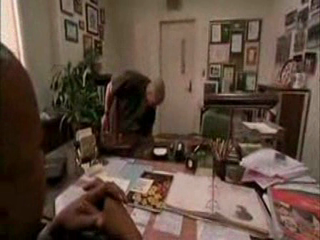
\includegraphics[width=3cm]{GolfFrames/B/00023.png}
		\label{fig:golf-comparison-b}
	}
	\subfigure[]{
		\includegraphics[width=3cm]{GolfFrames/C/00001.png}
		\includegraphics[width=3cm]{GolfFrames/C/00010.png}
		\includegraphics[width=3cm]{GolfFrames/C/00020.png}
		\includegraphics[width=3cm]{GolfFrames/C/00030.png}
		\label{fig:golf-comparison-c}
	}
	\centering
	\caption{Three examples of the $Golf$ class from the JHMDB dataset. The frames selected were four frames roughly evenly spaced out through the video.}
	\label{fig:golf-comparison}
\end{figure}

\begin{figure}[H]
	\subfigure[Precision]{
		\includegraphics[width=0.6\textwidth]{detailedPrecision}
	}
	\subfigure[Recall]{
		\includegraphics[width=0.6\textwidth]{detailedRecall}
	}
	\centering
	\caption{Detailed precision \& recall results on the JHMDB dataset, averaged over the 3 testing splits. Black bars show the corresponding maximum \& minimum values attained in one of the splits.}
	\label{fig:detailed-recall-precision}
\end{figure}

The detailed precision and recall values broken down by class are shown in figure \ref{fig:detailed-recall-precision}, and in general reflect the same results as the F1 scores. The only notable difference is the model tends to have more volatile recall whereas precision tends to be closer from one class to another. This can be seen more clearly in classes such as golf, pour, pullup, and push which have a very high recall compared to some other classes, but the precision is closer when compared to the other classes.

\afterpage{
	\begin{figure}[H]
		\subfigure[Split 1]{
			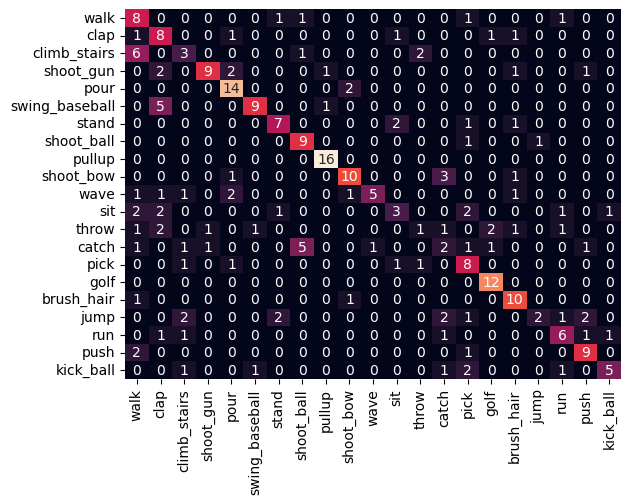
\includegraphics[width=0.6\textwidth]{confmatrix1}
		}
		\subfigure[Split 2]{
			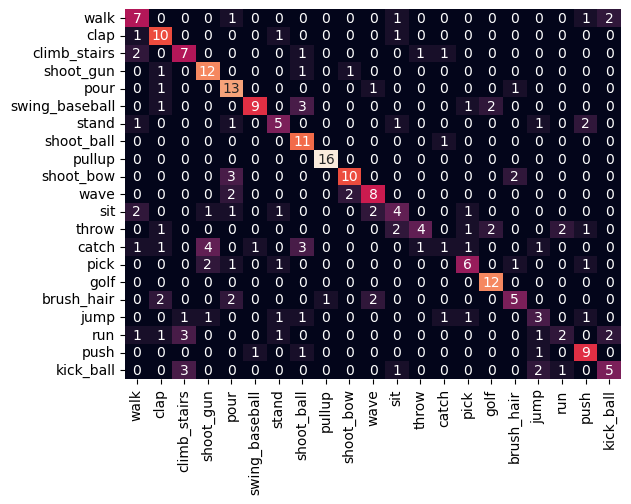
\includegraphics[width=0.6\textwidth]{confmatrix2}
		}
		\subfigure[Split 3]{
			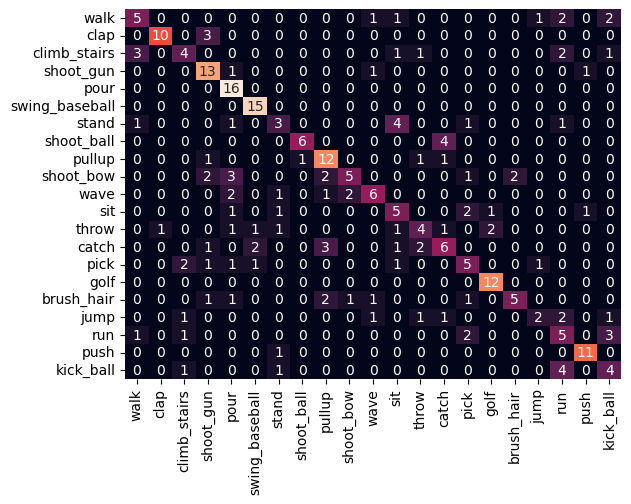
\includegraphics[width=0.6\textwidth]{confmatrix3}
		}
		\centering
		\caption{Confusion matrices for each of the 3 JHMDB splits.}
		\label{fig:confusion-matrices}
	\end{figure}
}

We can further explore the results as shown in figure \ref{fig:confusion-matrices}. These matrices for each split demonstrate that overall, the model predicts the correct class quite well. However it does tend to get confused in particular cases when the actions are similar, this will be further explained in when we study the failure cases in the next section.

\section{Failure Cases}
\label{sec:failure-cases}

There are some specific failure cases that are worth observing, similar to the example shown in figure \ref{fig:jump-comparison}. These failure cases are important to understanding how the model uses the representation and further examining the types of actions that the model has difficulty with outside of the previously discussed high variability in some actions.

\begin{figure}[ht]
	\includegraphics[width=3cm]{FailureCases/Catch/00001.png}
	\includegraphics[width=3cm]{FailureCases/Catch/00005.png}
	\includegraphics[width=3cm]{FailureCases/Catch/00010.png}
	\includegraphics[width=3cm]{FailureCases/Catch/00015.png}
	\centering
	\caption{An example of the \textbf{catch} action from the JHMDB dataset \cite{JHMDB}.}
	\label{fig:catch-action}
\end{figure}

Figure \ref{fig:catch-action} shows an example of the catch action. The primary issue is that throughout the four frames, there is very little movement by the main person who is performing the action of catching the ball. Due to the fact that the representation relies heavily on movement from one frame to another, this means that about 50\% of the representation is not used effectively because there is not very much movement. The underlying issue is that the model cannot see any person-object interactions. Other models that process the RGB frames or optical flow are able to pick up on the ball moving from one person to another, whereas our model cannot detect this object.

\begin{figure}[ht]
	\includegraphics[width=3cm]{FailureCases/Sit/00001.png}
	\includegraphics[width=3cm]{FailureCases/Sit/00010.png}
	\includegraphics[width=3cm]{FailureCases/Sit/00020.png}
	\includegraphics[width=3cm]{FailureCases/Sit/00030.png}
	\centering
	\caption{An example of the \textbf{sit} action from the JHMDB dataset \cite{JHMDB}.}
	\label{fig:sit-action}
\end{figure}

Another problem class is the sit action shown in figure \ref{fig:sit-action}. Our representation is designed in a way such that global position is not considered, which is an intentional decision in order to add some more ability for the model to generalize. This however also has some other consequences, as can be seen by the given example. The person does not have very much movement in their upper body, only pivoting at the hip. The crucial note that they are performing a "sit" rather than another action is their movement down through the frame. This global position change is not detectable by our representation and results in the model performing poorly for this class.

\begin{figure}[ht]
	\subfigure[]{
		\includegraphics[width=3cm]{FailureCases/Walk/00001.png}
		\includegraphics[width=3cm]{FailureCases/Walk/00015.png}
		\includegraphics[width=3cm]{FailureCases/Walk/00030.png}
		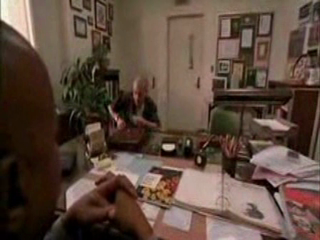
\includegraphics[width=3cm]{FailureCases/Walk/00040.png}
		\label{fig:run-action}
	}
	\subfigure[]{
		\includegraphics[width=3cm]{FailureCases/ClimbStairs/00001.png}
		\includegraphics[width=3cm]{FailureCases/ClimbStairs/00010.png}
		\includegraphics[width=3cm]{FailureCases/ClimbStairs/00020.png}
		\includegraphics[width=3cm]{FailureCases/ClimbStairs/00030.png}
		\label{fig:climb-action}
	}
	\centering
	\caption{Comparison between the \textbf{walk} (a) and \textbf{climb stairs} (b) actions from the JHMDB dataset \cite{JHMDB} showing similar movements.}
	\label{fig:walk-climb-actions}
\end{figure}

While the variability of actions is generally considered good for accuracy, this can also be detrimental to the performance of the model if two actions have very similar movements. This is shown in figure \ref{fig:walk-climb-actions}, where the actions shown (walk and climb stairs) have very similar movements. They differ only in two aspects. First, the climb stairs action generally moves the person vertically through the frame throughout. Second is that there are context clues in the background such as a lack of staircase in the run action, whereas the climb stairs action always has a staircase. In both of these cases, our model is not able to take this information in, resulting in the run and climb stairs actions looking similar in our representation, and making it difficult to distinguish between the two, resulting in the poor performance for both classes. As stated previously, this effect can be seen more in detail in figure \ref{fig:confusion-matrices}, where it is shown that the model quite often confuses climb stairs and walk.

\section{Model Ablation Study}

This section will present both different intermediate representation formats, as well as different model architectures. The natural first step to determining how effective the chosen architecture compared to others is to isolate each of the two halves (angle velocities \& angles themselves). These results are presented in tables \ref{tab:acc-results-v-velocity} and \ref{tab:acc-results-v-angle}.

\begin{table}[ht]
	\centering
	\begin{tabular}{||c c c||} 
		\hline
		\textbf{Split} & \textbf{Stacked} & \textbf{Only Angle Velocity} \\ [0.5ex] 
		\hline\hline
		1 & \textbf{58.209\%} & 48.888\% \\ 
		\hline
		2 & \textbf{58.889\%} & 44.444\% \\
		\hline
		3 & \textbf{58.113\%} & 41.132\% \\
		\hline
		\hline
		\textbf{Average} & \textbf{58.404\%} & 44.821\% \\
		\hline
	\end{tabular}
	\caption{Comparison of results using only angle velocities vs the stacked representation.}
	\label{tab:acc-results-v-velocity}
\end{table}

\begin{figure}[ht]
	\includegraphics[width=10cm]{detailedF1OnlyChange}
	\centering
	\caption{Detailed F1 score results on the JHMDB dataset using only the angle velocities from one frame to another.}
	\label{fig:detailed-f1-only-change}
\end{figure}

The only angle velocity results show an average decrease in performance over all three splits of approximately 14\% over the combination of the two. This is a very large decrease in accuracy, but is far from a negative result. What this result shows is that for some classes, the actual movement of the joint can be used in place of the joint angles and it is not necessarily required to have both in the representation. This is shown in figure \ref{fig:detailed-f1-only-change}, where we see that classes such as golf \& pullup still have a relatively high F1-Score of 0.7 on average.

\begin{table}[ht]
	\centering
	\begin{tabular}{||c c c||} 
		\hline
		\textbf{Split} & \textbf{Stacked} & \textbf{Only Angles} \\ [0.5ex] 
		\hline\hline
		1 & \textbf{58.209\%} & 56.343\% \\ 
		\hline
		2 & \textbf{58.889\%} & \textbf{58.889\%} \\
		\hline
		3 & \textbf{58.113\%} & 56.604\% \\
		\hline
		\hline
		\textbf{Average} & \textbf{58.404\%} & 57.279\% \\
		\hline
	\end{tabular}
	\caption{Comparison of results using only angles vs the stacked representation.}
	\label{tab:acc-results-v-angle}
\end{table}

Similarly, the representation that uses only angles and ignores the angle velocities shows a decrease in performance, as seen in table \ref{tab:acc-results-v-angle}. This is much less pronounced, and is only around 1\%. This suggests that while the angle velocities do add value, it is not uniformly a large positive. However when considering how small the added data is in the stacked representation the small increase in accuracy is justified.

Another intermediate representation was also explored as is shown in figure \ref{fig:alternating-intermediate}, where rather than "stacking" the angles and velocities on top of one another, we "interlace" the joint angles and their corresponding velocities. The idea behind this representation being that the initial CNN filters would overlap between each individual joint angle and their corresponding velocity, meaning that the model may be able to learn these relationships a bit better.

\begin{figure}[ht]
	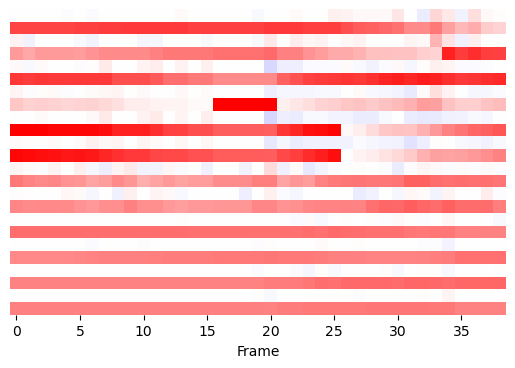
\includegraphics[width=0.5\textwidth]{IntermediateAlternatingFormat}
	\centering
	\caption{Alternative intermediate representation format where angles and velocities are interlaced rather than stacked.}
	\label{fig:alternating-intermediate}
\end{figure}

The results of this interlaced representation are shown in table \ref{tab:acc-results-v-alternating}. The results show on average a 4\% decrease in performance when compared to the stacked model. This is almost certainly because the model benefits more from the convolutions being run on the angles and velocities independently and combining later in the model after pooling layers rather than on both the angles and velocities initially.

\begin{table}[ht]
	\centering
	\begin{tabular}{||c c c||} 
		\hline
		\textbf{Split} & \textbf{Stacked} & \textbf{Interlacing} \\ [0.5ex] 
		\hline\hline
		1 & \textbf{58.209\%} & 54.850\% \\ 
		\hline
		2 & \textbf{58.889\%} & 55.556\% \\
		\hline
		3 & \textbf{58.113\%} & 52.830\% \\
		\hline
		\hline
		\textbf{Average} & \textbf{58.404\%} & 54.412\% \\
		\hline
	\end{tabular}
	\caption{Comparison of results using the interlacing vs stacked representation.}
	\label{tab:acc-results-v-alternating}
\end{table}

With this knowledge that the model typically performs better with the different features being stacked on top of each other and somewhat isolated, the next step was to see if further isolating the angles and velocities from one another would result in more performance gain. This resultant architecture is shown in figure \ref{fig:split-architecture}, where we split the angles and velocities completely, mimicking the fusion-based architectures as were shown previously in figure \ref{fig:fused}, where these models tended to split RGB, Optical Flow \& Pose data we similarly split our two pose joint features.

\begin{figure}[ht]
	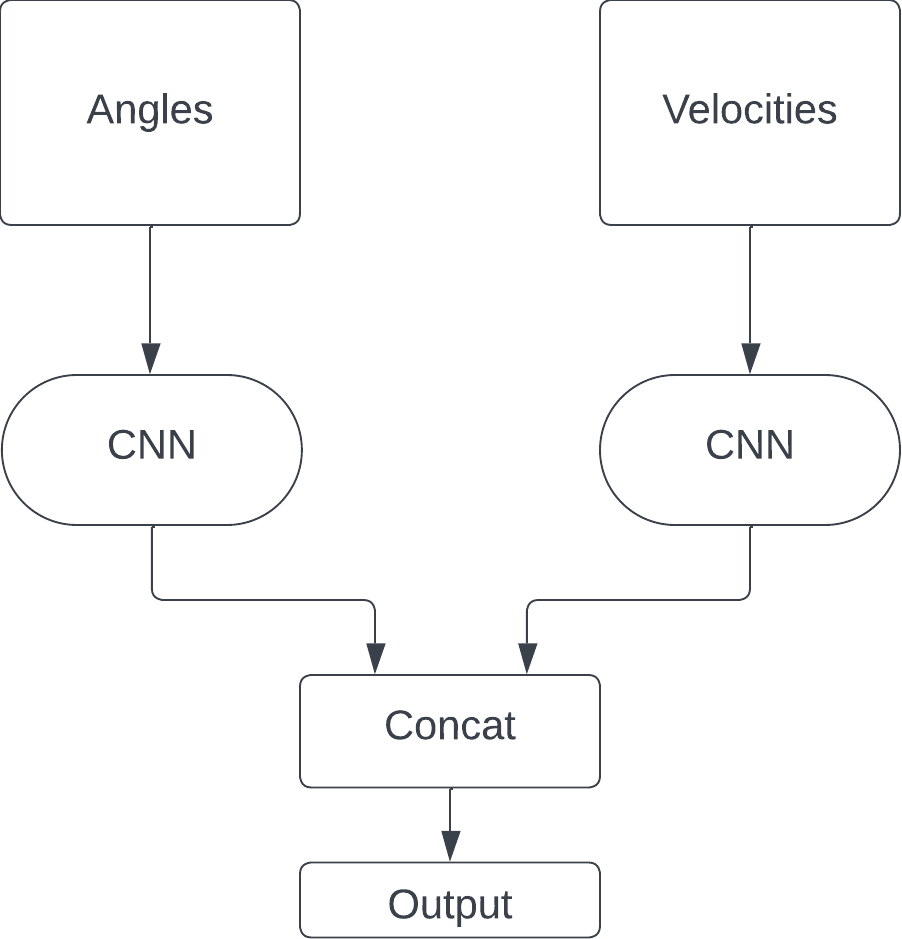
\includegraphics[width=0.4\textwidth]{SplitStructure}
	\centering
	\caption{The split model architecture inspired by fusion models where the two different pose features are split and utilize independent CNN's.}
	\label{fig:split-architecture}
\end{figure}

As can be seen from the results in table \ref{tab:acc-results-v-split}, once again this change to the model results in a decrease in performance by approximately 10\%. This reduction in performance is most likely because of the increase in complexity to the model, it overfit the relatively small dataset much more easily, meaning that it was less easily able to generalize. It may also be due to the fact that in the stacked representation, the combination of angles and velocities can be "learned" as the convolutions combine them at each step, whereas the split model isolates them until the very end, potentially losing data in the process.

\begin{table}[ht]
	\centering
	\begin{tabular}{||c c c||} 
		\hline
		\textbf{Split} & \textbf{Stacked} & \textbf{Split Representation} \\ [0.5ex] 
		\hline\hline
		1 & \textbf{58.209\%} & 46.269\% \\ 
		\hline
		2 & \textbf{58.889\%} & 48.889\% \\
		\hline
		3 & \textbf{58.113\%} & 49.811\% \\
		\hline
		\hline
		\textbf{Average} & \textbf{58.404\%} & 48.323\% \\
		\hline
	\end{tabular}
	\caption{Comparison of results using the split model and representation against the single CNN stacked representation.}
	\label{tab:acc-results-v-split}
\end{table}

We can also examine utilizing deeper and shallower networks with this representation. A shallower model would allow us to further reduction in memory needed to both rain the model as well as a reduction in the hardware required to run the model in production scenarios. A larger model could potentially allow for an increase in performance while sacrificing some of the advantages described previously. Table \ref{tab:acc-results-v-shallow-deep} shows these results, the results from both shallow \& deep models are outperformed by our proposed model. An exception is split 3 of the shallow model which outperforms our proposed model, however the average between the three splits is significantly lower. This is most likely due to the smaller model having slightly more volatility when it comes to each of the splits and results therefore varying more than our proposed model from one split to another.

\begin{table}[ht]
	\centering
	\begin{tabular}{||c c c c||} 
		\hline
		\textbf{Split} & \textbf{Standard Model} & \textbf{Shallow Model} & \textbf{Deep Model} \\ [0.5ex] 
		\hline\hline
		1 & \textbf{58.209\%} & 55.597\% & 55.970\% \\ 
		\hline
		2 & \textbf{58.889\%} & 57.407\% & 58.519\% \\
		\hline
		3 & 58.113\% & \textbf{59.245\%} & 53.585\% \\
		\hline
		\hline
		\textbf{Average} & \textbf{58.404\%} & 57.416\% & 56.025\% \\
		\hline
	\end{tabular}
	\caption{Comparison of results using the final model compared to a shallower model using one less convoultional layer group, as well as a deeper model containing one additional convolutional layer group.}
	\label{tab:acc-results-v-shallow-deep}
\end{table}

\section{Model Comparison}

When comparing our model and representation to others that are similar, it is important to note the difference in expected performance of our model vs. complex state of the art models. For this purposes of this thesis, we compare our model to other pose-based models, not taking into account those complex models that take very large GPU's to train, as this would be an unfair comparison.

\begin{table}[ht]
	\centering
	\begin{tabular}{||c c||} 
		\hline
		\textbf{Model} & \textbf{Average JHMDB Accuracy} \\
		\hline\hline
		Chained \cite{Chained} & 56.8\% \\
		Potion \cite{potion} & 57.0\% \\
		DynaMotion \cite{dynamic-motion} & 60.2\% \\
		EHPI \cite{simple_yet_efficient} & 60.5\% \\
		P-CNN \cite{PCNN} & 61.1\% \\
		SIP-Net \cite{sipnet} & 62.4\% \\
		STAR-Net \cite{star-net} & 64.3\% \\
		Pose \& Joint Aware \cite{poseandjointaware} & 68.55\% \\
		PA3D* \cite{PA3D} & 69.5\% \\
		Smaller, Faster, Better \cite{smaller_faster_better} & \textbf{77.2\%} \\
		\hline\hline
		\textbf{Ours} & 58.404\% \\
		\hline
	\end{tabular}
	\caption{Model comparisons that do not contain very complex models and utilize mainly pose data. * - PA3D uses additional data in it's representation as well.}
	\label{tab:model-comparison}
\end{table}

As can be seen from the results in table \ref{tab:model-comparison}, our model is not aiming to be the current state-of-the-art in it's category, however the performance is similar to the other models that approach the problem in a similar pose-based way. It is also notable, that our model is one of the only models that is both global position-invariant and scale-invariant, which is a large advantage of our model, and is by design as stated previously in this thesis.